\documentclass[12pt,english]{article}
\usepackage[cm]{fullpage}
\usepackage[utf8]{inputenc}
\usepackage[T1]{fontenc}
\usepackage{lmodern}
\usepackage[main=english]{babel}
\usepackage{mathtools}
\usepackage{siunitx}
\usepackage[dvipsnames]{xcolor}
\usepackage{listings}
\lstset{
	language=Python,
	morekeywords={as,assert,with},
	basicstyle=\footnotesize\ttfamily,
	keywordstyle=\bfseries\color{Plum},
	identifierstyle=\color{Red},
	stringstyle=\color{Green},
	commentstyle=\color{Gray},
	showstringspaces=false,
	tabsize=4,
	breaklines=true,
	prebreak=\mbox{\(\hookleftarrow\)},
	numbers=left,
	numberstyle=\footnotesize\color{darkgray},
	frame=leftline
}
\usepackage{tikz}
\usepackage[labelfont={bf},labelsep=endash]{caption}
\usepackage{hyperref}
\hypersetup{
	colorlinks=true,
	linkcolor=blue,
	urlcolor=cyan
}

\makeatletter
	\renewcommand*\and\\
	\let\old@itemize\itemize%
	\renewcommand\itemize{
		\parskip=0pt
		\old@itemize%
	}
	\let\old@enditemize\enditemize%
	\renewcommand\enditemize{
		\old@enditemize%
		\parskip=\baselineskip%
	}
	\let\old@enumerate\enumerate%
	\renewcommand\enumerate{
		\parskip=0pt
		\old@enumerate%
	}
	\let\old@endenumerate\endenumerate%
	\renewcommand\endenumerate{
		\old@endenumerate%
		\parskip=\baselineskip%
	}
	\renewcommand*\@maketitle{
		\begin{titlepage}
			\begin{flushright}
				ISEP
			\end{flushright}
			\begin{center}
				\vfill
				{\Huge\@title}

				\vspace{5cm}
				{\Large\@author}

				\vfill
				{\large\@date}
			\end{center}
		\end{titlepage}
	}
	\let\old@appendix\appendix
	\renewcommand*\appendix{
		\newpage
		\part*{Appendix}\addcontentsline{toc}{part}{Appendix}
		\old@appendix%
	}
	\addto\captionsenglish{
		\renewcommand\contentsname{Table of Contents}
	}
\makeatother

\author{
	Cyprien \textsc{Bariant} \texttt{10558}
	\and
	Tanguy \textsc{Berthoud} \texttt{60989}
	\and
	Thibault \textsc{du Buisson de Courson} \texttt{10496}
}
\title{
	\textbf{PROJECT}\\
	Advanced Algorithmic and Programming
}
\begin{document}
	\maketitle\newpage
	\thispagestyle{empty}
	\tableofcontents
	\listoffigures
	\listoftables
	\newpage
	\parskip=\baselineskip%

	\section{Creating a graph from GTFS data}\label{sec:step:1}
	\subsection{Importing relevant GTFS data}\label{sec:step:1.1}

	Our city of choice for the project is Phoenix, in Arizona.\\
	We use the public data available here: \url{https://transitfeeds.com/p/valley-metro/68/latest}

	The difficulty here was to import the relevant data and convert it to a graph.
	Some Python libraries seem to exist but none was convenient for the project, so we needed to transform the data manually.\\
	After reading documentation on GTFS, we needed only two files from the data feed: \texttt{stops.txt} and \texttt{stop\_times.txt}.

	\begin{center}
		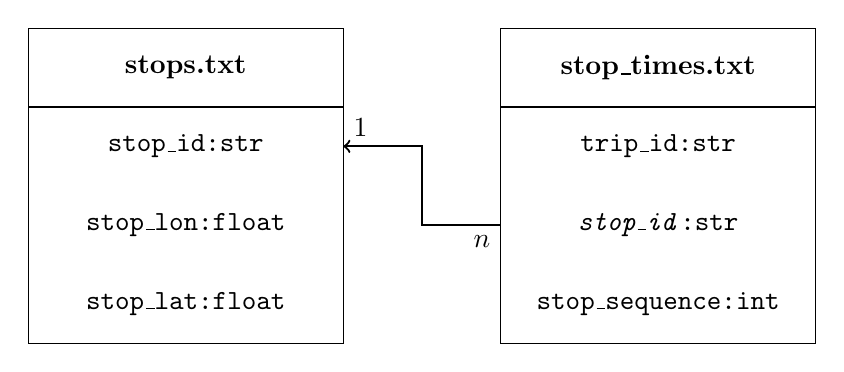
\begin{tikzpicture}
			\draw (0,3) rectangle +(4,1);
			\node at (2,3.5) {\bfseries stops.txt};
			\draw (0,0) rectangle +(4,4);
			\node at (2,2.5) {\ttfamily\bfseries stop\_id:str};
			\node at (2,1.5) {\ttfamily stop\_lon:float};
			\node at (2,.5) {\ttfamily stop\_lat:float};

			\draw (6,3) rectangle +(4,1);
			\node at (8,3.5) {\bfseries stop\_times.txt};
			\draw (6,0) rectangle +(4,4);
			\node at (8,2.5) {\ttfamily\bfseries trip\_id:str};
			\node at (8,1.5) {\ttfamily \textit{stop\_id}:str};
			\node at (8,.5) {\ttfamily stop\_sequence:int};

			\draw[thick,->] (6,1.5) node[anchor=north east] {\(n\)} -- ++(-1,0) -- ++(0,1) -- +(-1,0) node[anchor=south west] {\(1\)};
		\end{tikzpicture}
		\captionof{figure}{Database representation of the relevant GTFS files}
	\end{center}

	The nodes of the graph are directly given by the file \texttt{stops.txt}, so we can just parse the file to import them.
	This is done in the \texttt{import\_stops} function of \hyperref[sec:code:gtfs]{\ttfamily gtfs.py}.

	Whereas the edges need some operations:
	\begin{enumerate}
		\item Parse the file
		\item Regroup in order the stops in the same trips
		\item Create edges between consecutive stops in a trip
	\end{enumerate}
	This is done in the \texttt{import\_edges} function of \hyperref[sec:code:gtfs]{\ttfamily gtfs.py}.

	\subsection{Creating a graph}\label{sec:step:1.2}

	The \texttt{Graph} class is in \hyperref[sec:code:graph]{\ttfamily graph.py}.

	The class supports weighted directed graphs, but unweighted graphs can also be created.\\
	The class constructor accepts an optional parameter which is a callback to compute weight from two given nodes.
	In our case, this function takes two \texttt{Stop} (defined in \hyperref[sec:code:gtfs]{\ttfamily gtfs.py}) instances and returns the Euclidian distance between them: \[
		\text{compute\_weight}: (s,s') \mapsto \sqrt{\left(s'_\text{lat} - s_\text{lat}\right)^2 + \left(s'_\text{lon} - s_\text{lon}\right)^2}
	\]
	If this parameter is not passed, all edge weights will be set to \(0\).

	After testing the pathfinding methods (see \autoref{sec:step:2.2}), we realized that our way of storing neighbors was not optimized.\\
	Indeed we stored the neighbors in a huge adjacency list.
	So when we needed to compute some neighbors, we had to search in the whole list for neighbors.\\
	So we optimized this aspect.
	We are now storing the neighbors of a node inside the \texttt{Node} object itself.
	This implementation has redundancy in memory, but fetching the neighbors of a node is now \(\mathcal{O}(1)\) for the \texttt{neighbors\_out} and \texttt{neighbors\_in} methods.

	But our graph was just too big at that time to be able to work efficiently on it.\\
	So we restricted the graph to a district of the city, so the graph's order and size have been divided by 8.

	\subsection{Results}\label{sec:results:1}

	\begin{itemize}
		\item \(7982\) lines from \texttt{stops.txt} were imported to \(891\) nodes (\(7863\) before restricting the graph) in the graph.
		\item \(1720661\) lines from \texttt{stop\_times.txt} were imported to \(975\) edges (\(8319\) before the restriction) in the graph.
	\end{itemize}

	\begin{center}
		\begin{tabular}{r c c c}
			& \textbf{\ttfamily import\_stops} & \textbf{\ttfamily import\_edges} & \textbf{\ttfamily Graph}\\
			\hline\hline
			Before optimizations & \num{38.61} & \num{4211.02} & \num{78.64}\\
			& \num{31.75} & \num{5036.29} & \num{49.05}\\
			& \num{44.50} & \num{5085.64} & \num{68.83}\\
			& \num{28.56} & \num{3786.03} & \num{43.43}\\
			& \num{26.48} & \num{4070.86} & \num{43.62}\\
			\hline
			After neighbors optimization & \num{27.24} & \num{4931.54} & \num{155.09}\\
			& \num{29.34} & \num{3610.81} & \num{74.15}\\
			& \num{49.93} & \num{4096.88} & \num{115.51}\\
			& \num{28.70} & \num{3279.42} & \num{86.15}\\
			& \num{26.39} & \num{3685.92} & \num{82.94}\\
		\end{tabular}
		\captionof{table}{Execution time (\si{\milli\second}) for the graph creation over several tries}
		\label{tab:exectime:graph}
	\end{center}
	We see in this \autoref{tab:exectime:graph} that after the neighbors optimization described in \autoref{sec:step:1.2}, the execution time for the \texttt{Graph} instanciation has increased from an average of \SI{56.71}{\milli\second} to \SI{102.77}{\milli\second}.
	This can be explained by the new storage method of neighbors: we need to add two different tuples into two different sets.

	\section{Finding the shortest paths}\label{sec:step:2}
	\subsection{Common interface}\label{sec:step:2.1}

	To ease the usage of pathfinding for future computations, we created a common interface which is the \texttt{Pathfinder} class of \hyperref[sec:code:pathfinding]{\ttfamily pathfinding.py}.

	We used the \emph{Strategy design pattern} here with the \texttt{method} property, which is assigned in the class constructor to a function with the following signature: \[
		\text{method}: (\text{pathfinder}: \text{Pathfinder}, \text{start}: \text{int}) \rightarrow \text{None}
	\]
	This function is to compute all shortest paths from \texttt{start} and store them in \texttt{pathfinder}, using its \texttt{previous} and \texttt{distance} dictionnaries.

	\subsection{Pathfinding methods}\label{sec:step:2.2}

	We implemented two methods for the \hyperref[sec:step:2.1]{common interface}: \texttt{bfs} and \texttt{dijkstra}, defined in \hyperref[sec:code:pathfinding]{\ttfamily pathfinding.py}.

	Both use a queue to define the next nodes to be traversed, and proceed until this queue is empty.\\
	For \texttt{dijkstra}, this queue is actually a priority queue, sorted by ascending distance to \texttt{start}.

	For each outward neighbor \(n\) of the current traversed node \(c\), we initialize the relevant sections of \texttt{pathfinder} if needed, and we update them with the current neighbor traversed:
	\begin{itemize}
		\item[\texttt{bfs}] if \(d(\text{start},n) = d(\text{start},c) + 1\), then we add \(c\) to the backtrack list of \(n\).
		\item[\texttt{dijkstra}] if \(d(\text{start},n) \le d(\text{start},c) + w\) with \(w\) the weight of the edge \((c,n)\), then we add \(c\) to the backtrack list of \(n\). And if \(d(\text{start},n) < d(\text{start},c) + w\), then we reset the backtrack list and distance.
	\end{itemize}

	To optimize these methods, at the time when our graph was not restricted, we replaced the queues (which were simple lists) by heap queues using the \href{https://docs.python.org/3/library/heapq.html}{\ttfamily heapq} module of Python.\\
	This also improved the correctness of our methods, since it allows to pop nodes from the queue in a consistent order.

	\subsection{Results}\label{sec:results:2}

	\begin{center}
		\begin{tabular}{r c c}
			& \textbf{\ttfamily bfs} & \textbf{\ttfamily dijkstra}\\
			\hline\hline
			Before optimizations & \num{1.54} & \num{2.05}\\
			& \num{1.48} & \num{2.26}\\
			& \num{2.72} & \num{3.51}\\
			& \num{2.37} & \num{2.88}\\
			& \num{2.15} & \num{2.33}\\
			\hline
			After heaps optimization & \num{1.92} & \num{4.09}\\
			& \num{3.06} & \num{5.40}\\
			& \num{2.97} & \num{5.77}\\
			& \num{3.36} & \num{8.08}\\
			& \num{2.71} & \num{4.38}\\
		\end{tabular}
		\captionof{table}{Execution time (\si{\milli\second}) for the pathfinding methods over several tries}
		\label{tab:exectime:pathfinding}
	\end{center}
	We see in this \autoref{tab:exectime:pathfinding} that after the heaps optimization, the execution times have increased from an average of \SI{2.05}{\milli\second} to \SI{2.80}{\milli\second} for \texttt{bfs} and from \SI{2.61}{\milli\second} to \SI{5.54}{\milli\second} for \texttt{dijkstra}.
	Even though this optimization helped a lot when our graph was not restricted to a single district, it seems that using heap queues for little graphs does not help.

	\appendix

	This program is meant to be run by invoking Python on the \hyperref[sec:code:gtfs]{\ttfamily gtfs.py} script and adding the path to the GTFS data as argument.\\
	For example, you may execute \texttt{python src/gtfs.py ./data/} from the workspace root.

	\section{\texttt{gtfs.py}}\label{sec:code:gtfs}
	\lstinputlisting{../src/gtfs.py}

	\section{\texttt{graph.py}}\label{sec:code:graph}
	\lstinputlisting{../src/graph.py}

	\section{\texttt{pathfinding.py}}\label{sec:code:pathfinding}
	\lstinputlisting{../src/pathfinding.py}

	\section{\texttt{clustering.py}}\label{sec:code:clustering}
	\lstinputlisting{../src/clustering.py}
\end{document}
